\chapter{Method}\label{ch:method}

As mentioned above the approach in this project can be divided into two stages:

\begin{figure}[ht]
    \centering
    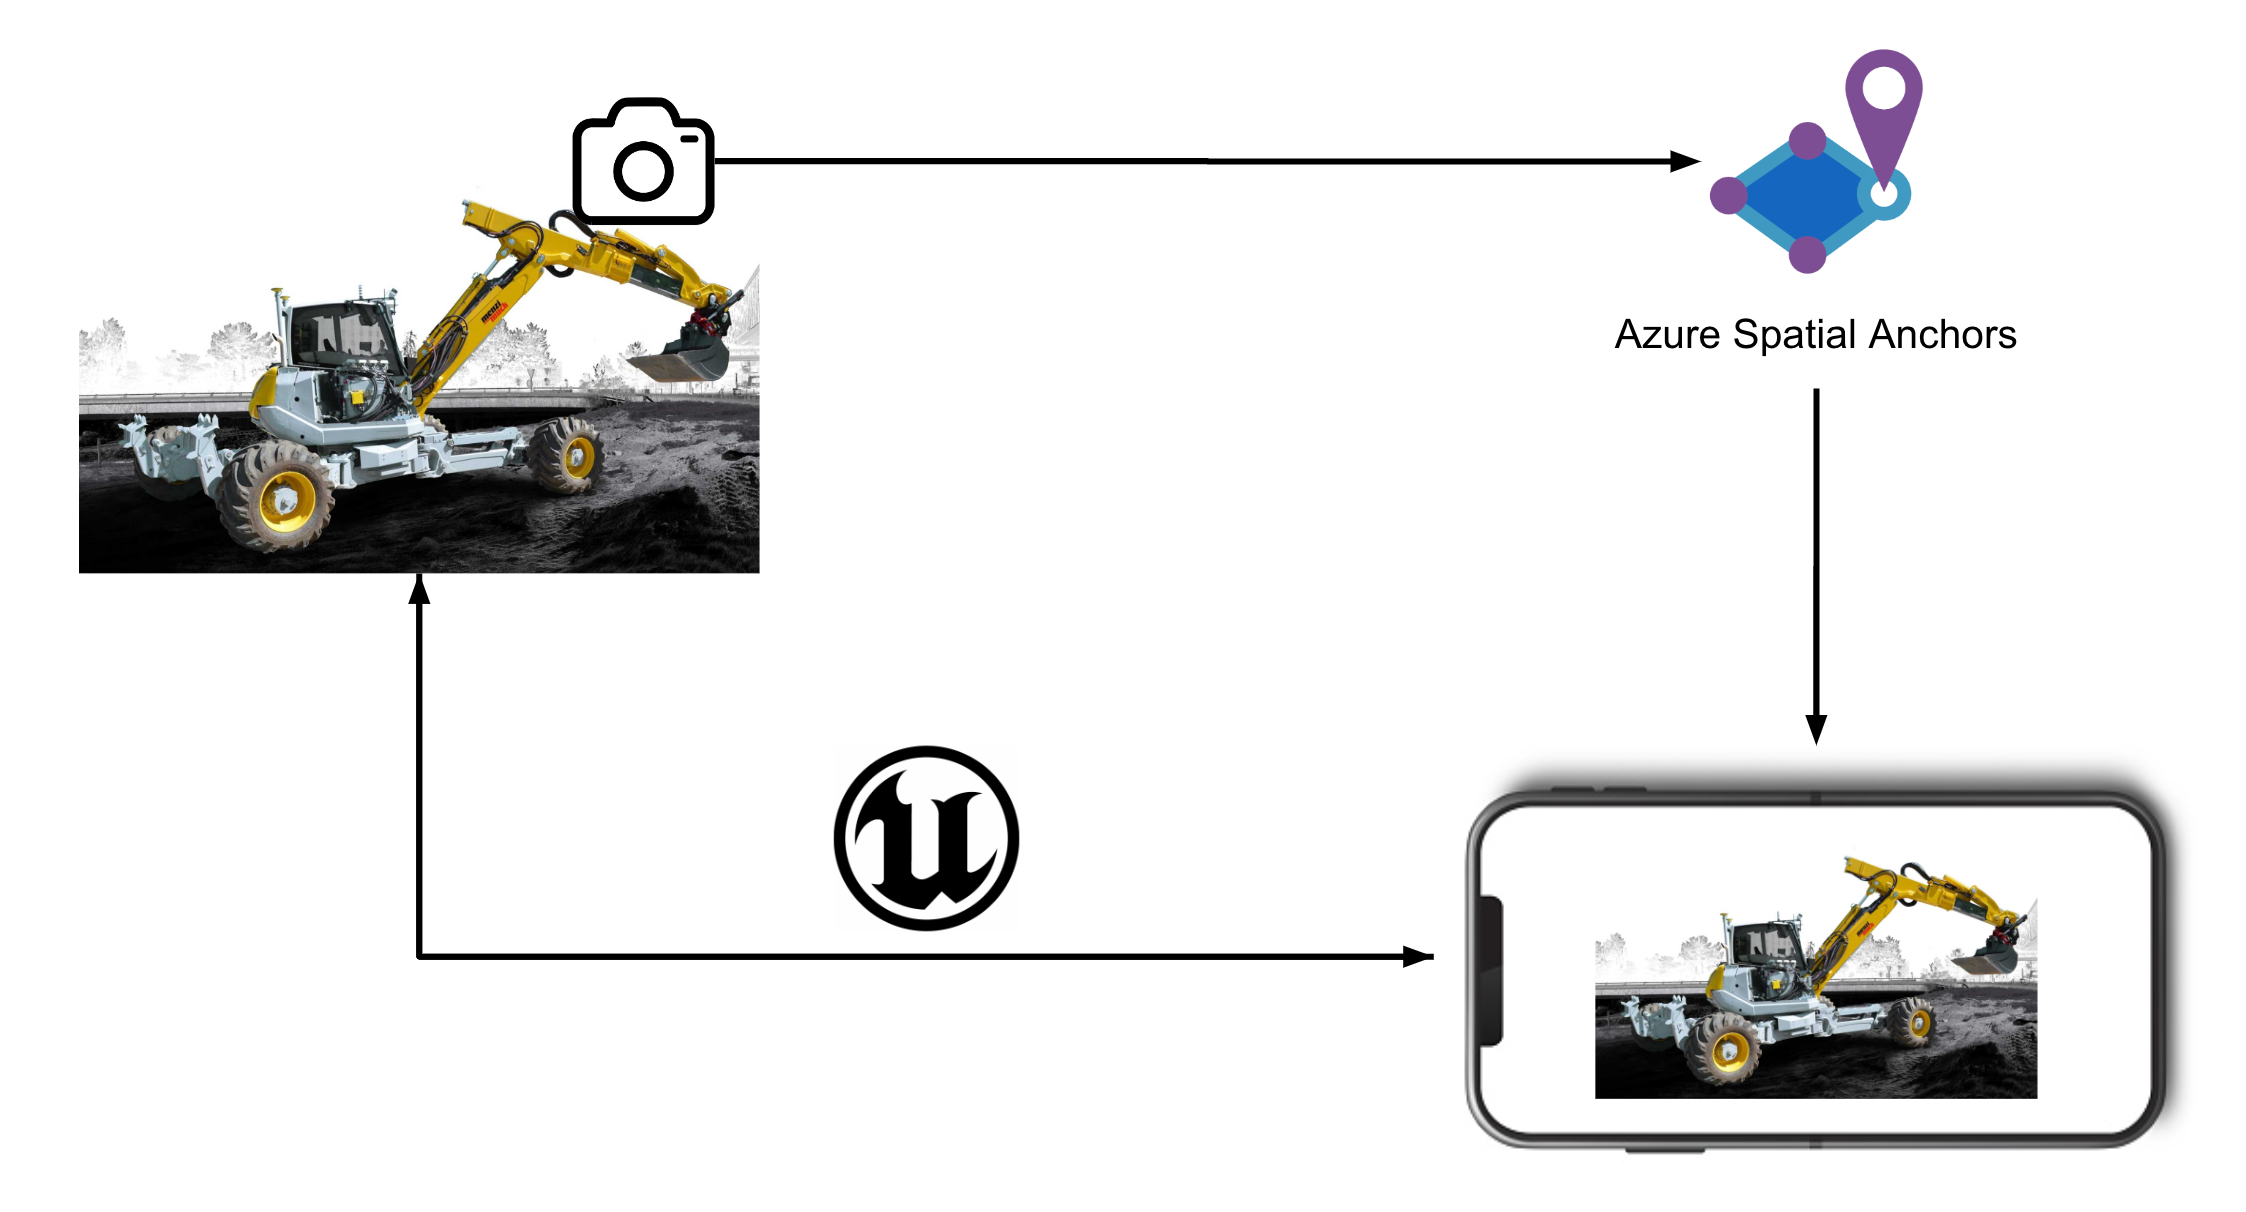
\includegraphics[scale = 0.32]{images/method/method.png}
    \caption{High level handheld remote setup}
    \label{fig:method}
\end{figure}

\begin{itemize}
    \item Data transfer between the excavator and the handheld device (left arrow connection)
    \begin{itemize}
        \item Creating an Augmented Reality Unreal Engine (UE) game on the handheld device
        \item Making use of the already existing UE interface on the excavator to store system information in game components 
        \item Using an Unreal Engine local multiplayer connection in order to transfer data between the two UE instances
    \end{itemize}
    \item Colocalization between the two frames of reference (right arrow connection) 
    \begin{itemize}
        \item Extracting a spatial anchor from the excavator's camera view using a ROS wrapper 
        \item Uploading this visual anchor in the form of an Azure Spatial Anchor to the Azure cloud
        \item Retrieving the stored spatial anchor in the handheld UE instance 
        \item Using the spatial anchor to relocate the UE world origin
    \end{itemize}
\end{itemize}




